\subsection{Concept of boundary layer}
	The motion of viscous environment is almost always associated with transfer phenomena in the boundary layer, where friction resistances, heat and mass transfer are localized. The concept of a boundary layer was first used by Ludwig Prandtl in an article presented on August 12, 1904, at the third International Congress of Mathematicians in Heidelberg, Germany. A classic example of a boundary layer is the boundary layer, which is formed on a flat plate when a liquid flows around its surface, and the boundary layer in round pipes. More difficult to study and mathematically describe is the boundary layer on surfaces with different curvature (flow around a cylinder, sphere, and other bodies). Such a boundary layer is characterized by a large pressure gradient and a separation point, beyond which the derivative and the flow velocity change signs. The boundary layers at the area between two-phase and multi-phase environments are also much more complex and difficult to access.
	
	Boundary layer -- the area of the flow of a viscous fluid with a small transverse thickness compared to the longitudinal dimensions, which is formed near the surface of a streamlined solid body or at the boundary between two fluid flows with different velocities or temperatures. The boundary layer is characterized by a sharp change in the transverse direction of velocity (dynamic boundary layer) or temperature (temperature boundary layer).
	
	The lower the viscosity of the medium, the thinner the hydrodynamic boundary layer and the greater the significance of the velocity gradient in this layer. Outside the boundary layer, the velocity gradient is small. Consequently, the friction forces here are small and are usually neglected. There is no sharp boundary between the external flow and the boundary layer, since the average fluid velocity over the flow cross section changes monotonically, without jumps. Usually, the thickness of the boundary layer is determined conditionally, based on the fact that at its outer boundary the velocity is 99\% of the velocity of the external flow.
	
	The value of the boundary layer is very important, since it determines the hydrodynamic resistance when the environment moves relative to the solid body, as well as the resistance to mass and heat transfer. The introduction of this concept significantly simplified the equations for modeling the fluid flow by dividing the flow into two regions.
	
	There are three types of flow in the boundary layer, each of which has its own characteristics and some of them are quite complex for numerical simulation:
	\begin{itemize}
		\item laminar -- the movement of the fluid is ordered, the layers do not mix, the particles rotate within the same thin layer;
		\item turbulent -- the motion is disordered, particles are mixed in the transverse direction and the entire boundary layer is randomly swirling;
		\item mixed -- transitional state from laminar to turbulent motion.
	\end{itemize}

	In the general case, the non-isothermal motion of a viscous compressible fluid is described by the following equations: the Navier-Stokes equations, the equation of continuity, convective heat conduction and state.
	\begin{align}
		& u\frac{\partial u}{\partial x} + v\frac{\partial u}{\partial y} + w\frac{\partial u}{\partial z} = -\frac{1}{\rho}\frac{\partial p}{\partial x} + \nu(\frac{\partial^2 u}{\partial x^2} + \frac{\partial^2 u}{\partial y^2} + \frac{\partial^2 u}{\partial z^2}) \nonumber\\
		& u\frac{\partial v}{\partial x} + v\frac{\partial v}{\partial y} + w\frac{\partial v}{\partial z} = -\frac{1}{\rho}\frac{\partial p}{\partial y} + \nu(\frac{\partial^2 v}{\partial x^2} + \frac{\partial^2 v}{\partial y^2} + \frac{\partial^2 v}{\partial z^2})\nonumber\\
		& u\frac{\partial w}{\partial x} + v\frac{\partial w}{\partial y} + w\frac{\partial w}{\partial z} = -\frac{1}{\rho}\frac{\partial p}{\partial z} + \nu(\frac{\partial^2 w}{\partial x^2} + \frac{\partial^2 w}{\partial y^2} + \frac{\partial^2 w}{\partial z^2})\nonumber\\
		& \frac{\partial u}{\partial x} + \frac{\partial v}{\partial y} + \frac{\partial w}{\partial z} = 0 \nonumber\\
		& \rho c (\frac{\partial T}{\partial\tau} + \vec{v}\nabla T) = div(\lambda grad(T)) + q_v + \mu\Phi - p div(\vec{v}) \nonumber\\
		& f(p, \rho, T) = 0
	\end{align}
	Based on this, we have 6 equations and 6 unknowns($u, v, w, \rho, T, p$). This system is extremely complex and, in general terms, is difficult to solve even by modern numerical methods on powerful PCs. Therefore, various simplifications of this system are often considered.


\subsection{Turbulent state of the boundary layer}
	Laminar flow is stable only under certain conditions determined by the value of the critical Reynolds number $Re_{cr}$. Usually, the transition from laminar to turbulent fluid flow in pipes is observed at $Re_{cr} \approx 2300$. Turbulent motion in the boundary layer arises from flow instability, which manifests itself in the form of vortices of various sizes and intensities. These vortices mix the liquid layers, which leads to an increase in the transfer of mass and energy along the surface of the solid. A turbulent flow with a large Reynolds number is called developed turbulence. If the pipe inlet is made smooth, then the laminar motion in the pipe can be maintained at high Reynolds numbers, for example up to 24000. Significantly affect at $Re_{cr}$ such factors as pressure gradient, channel shape, roughness of its walls, injection and suction of the boundary layer. An increase in pressure in the direction of motion leads to instability of the flow in the boundary layer, separation, and the appearance of vortices. Therefore, both for internal (in pipes and channels) and external (flow around bodies) flows, the critical Reynolds number increases with a decrease in the external pressure gradient (accelerating flows - according to Bernoulli's law).
	
	Turbulence can be defined as a three-dimensional unsteady motion in which, due to the stretching of vortices, a continuous distribution of velocity fluctuations is created in the range of wavelengths from the minimum, determined by viscous forces, to the maximum, determined by the boundary conditions of the flow. In the mathematical description of turbulent flows, it is convenient to proceed from the understanding of turbulence as a hierarchy of eddies of various scales, using the eddy and wave interpretation of turbulence\cite{Монин1992}. Turbulent eddies are continuous and constantly in contact with each other, and large eddies, the dimensions of which are determined by the boundary conditions of the problem, contain smaller eddies.
	
	The maximum size of vortices is close to the characteristic linear scale of the problem $L$. Often the motion of the largest vortices turns out to be largely ordered (for example, the flow behind a cylinder). Such structures are often called coherent. Vortices of the minimum size dissipate directly into heat. Their size is characterized by the Kolmogorov scale $(\nu^3/\epsilon)^{1/4}$. In this case, vortices of a certain average size carry the greatest amount of energy.
	
	One of the important characteristics describing turbulent motion is vorticity $\omega$: 
	\begin{align}
		\vec{\omega} = \vec{\nabla}\times \vec{v} \qquad \omega_x = \frac{\partial w}{\partial y} - \frac{\partial v}{\partial z}, \qquad \omega_y = \frac{\partial u}{\partial z} - \frac{\partial w}{\partial x}, \qquad \omega_z = \frac{\partial v}{\partial x} - \frac{\partial u}{\partial y}
	\end{align}

\subsection{Boundary layer structure}
	Ideas about the structure of the velocity profile gradually changed and were finally formed by the end of the 1950s. In a turbulent boundary layer, several regions are usually distinguished: external and internal. They differ from each other by different scales of vortex structures.\cite{Белов2001}.
	\begin{figure}[H]
		\centering
		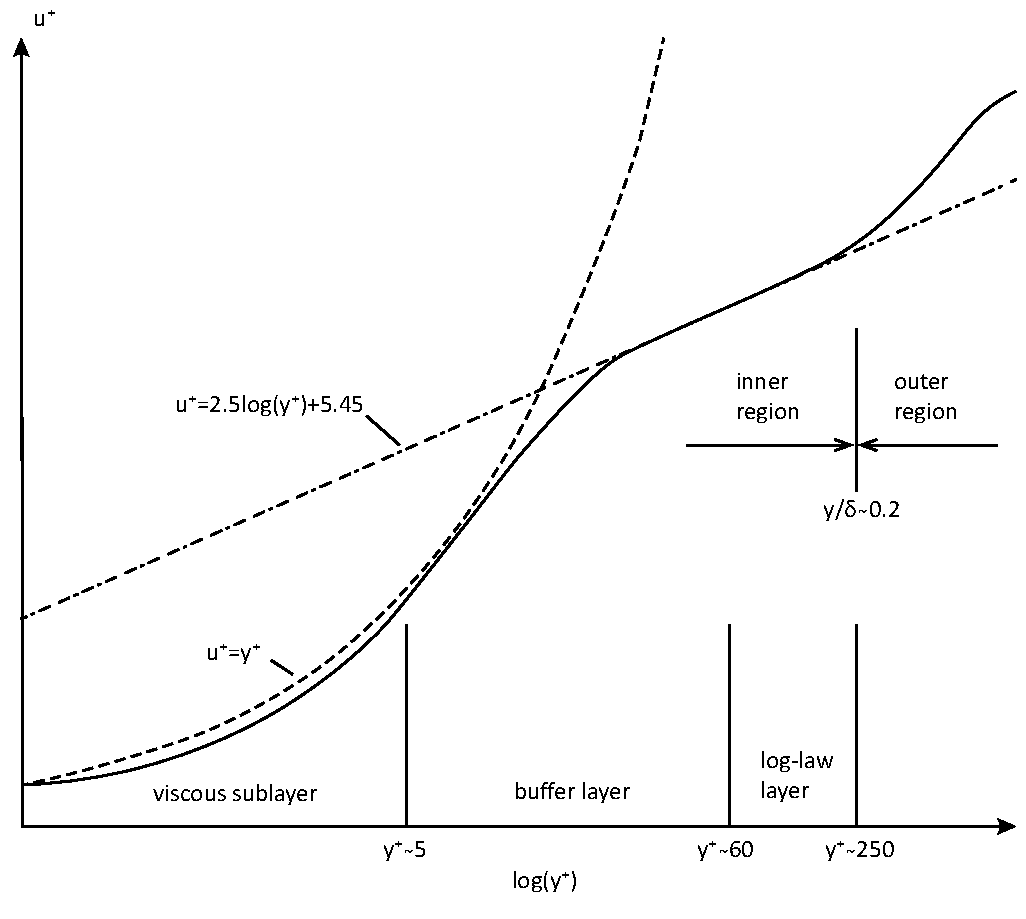
\includegraphics[width=0.7\linewidth]{../Assets/ПогранСлойEN}
		\caption{\footnotesize {Layer structure}}
	\end{figure}
	The inner region of the boundary layer occupies approximately 20\% of the thickness of the entire layer and generates up to 80\% of the turbulence energy in it. The formation of flow in the boundary layer is mainly influenced by the viscosity, thermal conductivity, and diffusion capacity of the liquid. Inside the dynamic boundary layer, there is a smooth change in velocity from its value in the external flow to zero on the wall due to the adhesion of a viscous fluid to a solid surface. Similarly, the temperature changes smoothly inside the boundary layer.

\subsubsection{Outer area}
	The outer layer is an area of fully developed turbulent flow, in which the velocity distribution is described by a logarithmic law. Complete damping of perturbations in the outer region occurs at a distance many times greater than the linear scale of turbulence.
	
	The filtered or Reynolds-averaged Navier-Stokes equations are used to determine the flux in the outer zone. At the same time, the velocity profile in the inner zone depends relatively little on various external conditions, such as Reynolds numbers and pressure gradient, which makes it possible to use universal relations (wall functions) to relate the flow parameters to the distance from the wall. This method is also based on the hypothesis of local equilibrium of the energy of turbulent fluctuations and the local isotropy properties of dissipating vortices

\subsubsection{Inner area}
	The viscous sublayer, buffer and logarithmic layers make up the inner region of the boundary layer. It is characterized by a high rate of mass, momentum and heat transfer, resulting in increased friction and energy loss.
	\begin{align}
		v\frac{\partial u}{\partial y} \gg -\overline{u'v'} & \qquad\text{viscous}\nonumber \\
		v\frac{\partial u}{\partial y} \approx -\overline{u'v'} & \qquad\text{buffer}\nonumber \\
		v\frac{\partial u}{\partial y} \ll -\overline{u'v'} & \qquad\text{logarithmic}
	\end{align}

	There are two approaches to modeling the flow in the near-wall region. In the first approach, semi-empirical formulas (wall functions) are used to describe the inner layer of the flow, while in the second approach, the turbulence models are modified in such a way as to resolve the entire near-wall region of the flow, including the viscous sublayer, provided that the required grid resolution in the boundary layer is provided. Such turbulence models can be used to calculate turbulent flows in the entire computational domain (including the near-wall flow region).
	
\subsubsection{Boundary layer properties}
	The thickness of the boundary layer is difficult to determine both in the calculation and in the experiment. The following concepts are used to define: displacement thickness $\delta^*$ and momentum loss thickness $\theta$.
	\begin{equation}
		\delta^* = \int_{0}^{\infty}(1 - \frac{u}{U_0})dy \qquad \theta = \delta^{**} = \int_{0}^{\infty} \frac{u}{U_0}(1 - \frac{u}{U_0})dy
	\end{equation}

	In addition, the dimensionless parameter is used $H$:
	\begin{equation}
		H = \frac{\delta^*}{\theta}
	\end{equation}

	The Reynolds number is characterized by two quantities($Re_x$ и $Re_\theta$): distance from bottom wall $x$ and thickness $\theta$.
	\begin{equation}
		Re_x = \frac{xU_0}{\nu} \qquad Re_\theta = \frac{\theta U_0}{\nu}
	\end{equation}

	Using the friction stress on the wall $\tau_w$ we can calculate the coefficient of friction $C_F$ and dynamic velocity $u_\tau$:
	\begin{equation}
		\tau_w = \nu\frac{\partial u}{\partial y}\bigg|_W \qquad C_F = \frac{\tau_w}{0.5\rho U_0^2} \qquad u_\tau = \sqrt{\frac{\tau_w}{\rho}}
	\end{equation}
	
	An equally important characteristic of the boundary layers is the longitudinal pressure gradient:
	\begin{equation}
		\frac{dp}{dx} = -\rho U_0 \frac{dU_0}{dx}
	\end{equation}
	
	Boundary layers are often affected by the following factors: surface curvature $\kappa$, liquid pumping and pumping speed, surface roughness $k_s^+$(height of hillocks).
	\begin{equation}
		\kappa = \frac{\delta^*}{R} \qquad \frac{V_W}{u_\tau}, \frac{V_W}{U_0} \qquad k_s^+ = \frac{k_s u_\tau}{\nu}
	\end{equation}

	An important property of the boundary layer is the fulfillment of the integral momentum equation. The converse is also true: if the momentum ratio is not high, then the flat boundary layer equation is also not true for the flow. This may be the influence of the aggregate: the three-dimension of the flow, its non-stationarity, the influence of the increase in flow, the change in pressure across the boundary layer, the influence of normal Reynolds surges, etc.
	\begin{equation}
		\frac{d\theta}{dx} + \frac{dU_0}{dx}\cdot\frac{2 + H}{U_0}\theta - \frac{C_f}{2} = 0
	\end{equation}
	
\subsection{Local friction and transport}
	The theoretical basis for describing the transfer processes in the boundary layer is the fundamental laws of conservation and equilibrium, one of the properties of which is their invariance to scale and interaction with other phenomena, i.e. the structure of the mathematical description of the boundary layer weakly depends on the contact device.
	
	To study the effect of vortex generators in a turbulent boundary layer on local friction and transfer, the following parameters were studied: average velocity and its pulsation , friction stress on the wall $\tau_w$, coefficient of friction $C_F$, and dynamic velocity $u_\tau$. To represent the profiles of the mean velocity components and their fluctuations, dimensionless coordinates were used $u^+$ и $y^+$:
	\begin{equation}
		u^+ = \frac{U}{u_\tau} \qquad y^+ = \frac{yu_\tau}{v}
	\end{equation}

\subsection{Modeling methods}
	Despite the intensive development of computer technology and the impressive progress achieved in recent years both in the field of constructing efficient numerical algorithms designed to solve problems of hydromechanics and heat and mass transfer, and in the development of related software (mesh generators, interactive data entry systems and systems for visualizing the results of calculations ), the problem of numerical simulation of turbulence, as it has been for many previous decades, still remains one of the most complex and urgent problems of fluid mechanics. Unlike laminar flows of a single-phase medium (liquid), the calculation of which, thanks to the achievements noted above, has become largely a routine procedure, reliable prediction of the characteristics of complex turbulent flows, which are of the greatest practical interest, is still difficult.
	\begin{figure}[H]
		\centering
		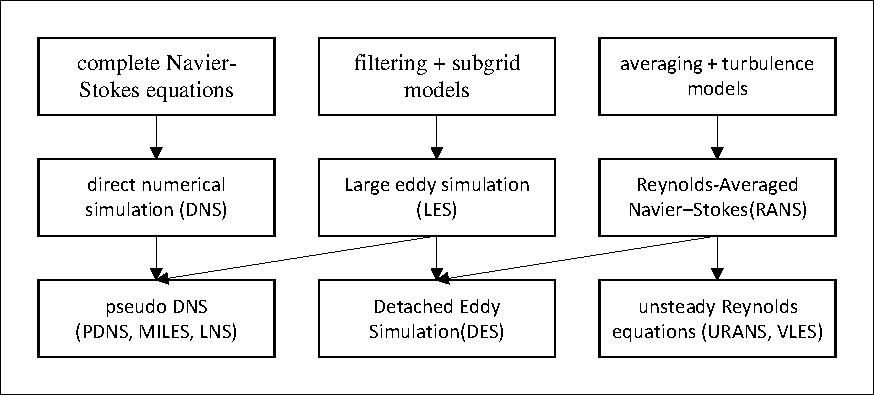
\includegraphics[width=0.9\linewidth]{../Assets/СхемаМетодовEN}
		\caption{\footnotesize{Types of methods by equations}}
		\label{fig:cheme}
	\end{figure}
	
	Among the main methods of numerical simulation of three-dimensional turbulent flows are: direct numerical simulation (DNS), simulation of large eddies (LES) and solution of Reynolds-averaged Navier-Stokes equations (RANS). There are also various intermediate approaches that combine certain features of RANS, LES, and DNS, for example, the detached eddy modeling method (DES), and a number of others that do not have a proper physical justification and, therefore, are not widely used.
	
\subsubsection{DNS}
	Direct numerical simulation (DNS) involves solving the complete non-stationary three-dimensional Navier-Stokes equations, which makes it possible to obtain instantaneous characteristics of a turbulent flow. Problems with the widespread use of the DNS are associated with high requirements for the difference scheme used, satisfaction of the initial and boundary conditions, as well as limited computing resources. In this case, the computational domain should be sufficiently extended to accommodate the largest scales of turbulence, and the time integration step should be of the order of the Kolmogorov scale.
	\begin{table}[H]
		\begin{center}
			\begin{tabular}{|c|c|c|c|c|}
				\hline
				Re & 6.6$\times10^3$ & 2.0$\times10^4$ & 1.0$\times10^5$ & 1.0$\times10^6$\\
				\hline
				Number of nodes & 2$\times10^6$ & 4$\times10^7$ & 3$\times10^8$ & 1.5$\times10^3$\\
				\hline
				150 MFlops & 37 h & 740 h & 6.5 years & 3000 years\\
				\hline
				1 TFlops & 20 s & 400 s & 8.3 h & 4000 h\\
				\hline
			\end{tabular}
		\end{center}
		\caption{\footnotesize{Time spent for various parameters}}
	\end{table}
	
	These stringent requirements are partly relaxed by using high-precision spectral methods for the numerical integration of the Navier-Stokes equations, which are often used for DNS. However, these methods are not applicable to the calculation of flows with complex geometry. These circumstances lead to the fact that in practice the DNS is used only for calculating simple turbulent flows at low Reynolds numbers. In this case, the main task of the calculation is not actually obtaining data on the characteristics of the averaged flow (they are usually known), but obtaining detailed information about the structure of turbulence, as well as calculating individual terms included in certain turbulence models.
	
\subsubsection{RANS}
	Mathematical models based on the numerical solution of the Reynolds-averaged Navier-Stokes (RANS) equations are widely used in engineering applications. When using the Reynolds equations, the main interest is in the dynamics of large-scale eddies responsible for the transport properties of turbulent flows. When closing the Reynolds equations, we consider length scales typical of energy-containing vortices, in which $Re\gg1$ (except for near-wall areas). To take into account the near-wall influence of dissipating vortices and energy-containing vortices at $Re\sim1$ damping functions are used. Applying the Reynolds averaging to the equations, we obtain:
	\begin{align}
		&\frac{\partial u_i}{\partial x_i} = 0 \nonumber\\
		&\rho\frac{\partial u_i}{\partial t} + \rho u_j \frac{\partial u_i}{\partial x_j} = - \frac{\partial p}{\partial x_i} + \frac{\partial}{\partial x_j}(\mu\frac{\partial u_i}{\partial x_j} - \rho\overline{u_i' u_j'})
	\end{align}
	This system is not closed, since it includes an unknown tensor of the so-called Reynolds stresses $\tau_{ij} = -\rho\overline{u_i' u_j'}$(turbulent stresses). To close this system of equations, it is necessary to determine six different components of the symmetric turbulent stress tensor. It is the expression of these components in terms of the average flow parameters that is called the turbulence model. Below is a table with the main stages in the development of the theory.
	
	\begin{table}[H]
		\begin{center}
			\begin{tabular}{|c|c|c|}
				\hline
				Year & Scientist & Study\\
				\hline
				1877 & Boussinesq J. V. & Boussinesq conjecture\\
				\hline
				1895 & Reynolds O. & Reynolds averaging\\
				\hline
				1925 & Prandtl L. & Prandtl's mixing path theory\\
				\hline
				1930 & Theodore von Karman & Karman's formula\\
				\hline
				1942 & Kolmogorov A. N. & Kolmogorov formula, model $k$-$\omega$\\
				\hline
				1951 & Rotta & first Reynolds stress model\\
				\hline
				1956 & Clauser & Clauser formula\\
				\hline
				1956 & Driest E. R. & damping factor\\
				\hline
				1974 & Launder B. E.and Spalding D. B & model $k$-$\epsilon$\\
				\hline
			\end{tabular}
		\end{center}
		\caption{\footnotesize{Stages of development of the theory}}
	\end{table}
	
	The emergence of a huge number of models has led to the need of choice. To do this, it is necessary to conduct a comparative analysis of models. However, when trying to test in a natural way, certain difficulties arise. First, it is necessary to choose flows for which a set of reliable experimental data is known, free from errors, and also to choose criteria for comparing models. Secondly, it is necessary to carry out serial calculations of these flows using different turbulence models and, at the same time, be sure that the result is independent of the software implementation of the problem. The result of such work should be recommendations on the area of applicability of certain turbulence models.
	
\subsubsection{LES}
	The large eddy simulation method (LES) was proposed by Iosif Smagorinsky in 1963. It is based on two assumptions. The first assumes that the flow can be divided into the movement of large and small eddies. Large eddies that are under the direct influence of boundary conditions and carry the maximum of Reynolds stresses are calculated. Small-scale turbulence is considered to be isotropic and have universal characteristics, and therefore less critical and more amenable to modeling. Another is the possibility of approximating the nonlinear interactions between large and small eddies only by large eddies using subgrid models (SGS). In other words, the hypothesis of the statistical independence of large and small eddies is accepted.
	
	Large eddy statistics are usually insensitive to subgrid simulations, except for the near-wall region. Available subgrid models correctly predict not only averaged flow characteristics (first and second moments), but also fluctuations of integral characteristics, such as drag and lift coefficients\cite{Fureby2000}. Small-scale motion is eliminated from the Navier-Stokes equations by applying a filtering operation and modeled using subgrid models. On the image \ref{fig:lesfilter} the principle of operation of filters is shown, where $g(x)$ - original version, $f(x)$ - after filtration.\\
	\begin{figure}[H]
		\centering
		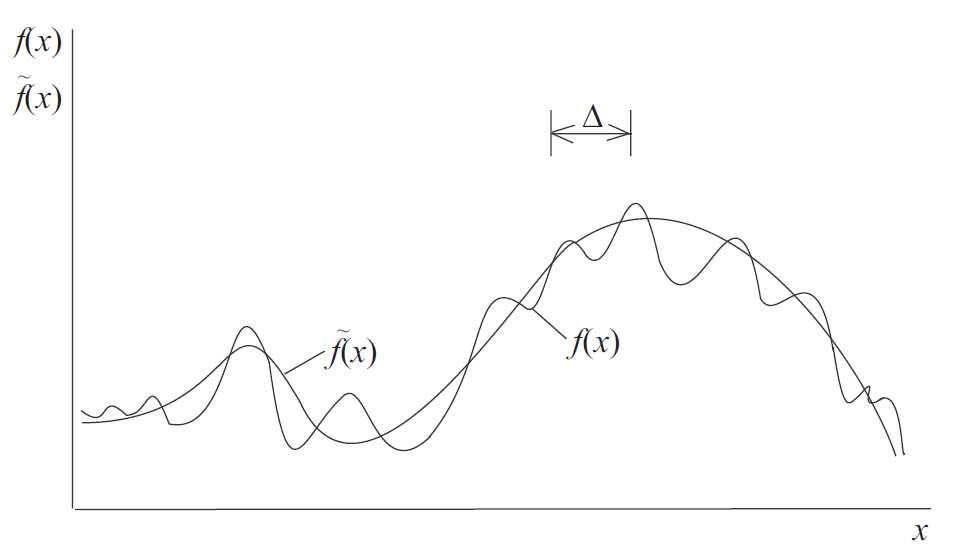
\includegraphics[width=0.7\linewidth]{../Assets/ФильтрацияLES}
		\caption{\footnotesize{Exclusion of small-scale motions by filtering}}
		\label{fig:lesfilter}
	\end{figure}

	Filter equation applied to the space-time field $\phi(x,t)$ presented below:
	\begin{equation}
		\overline{\phi(x,t)} = \int_{-\infty}^{\infty}\int_{-\infty}^{\infty}\phi(r,t')G(x - r, t - t')dt'dr
	\end{equation}
	In this case, $G$ is a kernel specific to each type of filter.
	
	The LES solution contains richer information than the Reynolds equation solution, for example, not only mean flow characteristics (velocity, concentration, temperature, pressure fields) and Reynolds stress distributions, but also spectral characteristics (pulsation spectra velocity and pressure), two-point moments, temporal and spatial scales of turbulence.
	
\subsubsection{DES}
	Large-scale unsteady three-dimensional vortex structures characteristic of separated flows are determined by specific boundary conditions and geometric characteristics of the flows under consideration and cannot be described within the framework of such models. This stimulates the search and development of hybrid approaches that combine the cost-effectiveness of RANS and the versatility of LES.
	
	In the detached eddy modeling (DES) method, in the region of the attached boundary layer, the method operates in the Reynolds equations mode, and in the region of flow separation it passes into LES. In this case, a combination of the best qualities of both approaches is achieved - the high accuracy and efficiency of the Reynolds equations in the region of the attached boundary layer and the universality of LES in the separation region. Although DES, unlike RANS, is a fundamentally non-stationary three-dimensional approach, the grids in the near-wall region required for its implementation coincide with the grids necessary for solving the Reynolds equations and are many orders of magnitude smaller than the grids required for resolving small near-wall vortices in the framework of LES. As the grid refines, DES asymptotically approaches LES and further to DNS. Specific implementations of DES are based on the use of the Spalart-Allmaras turbulent viscosity model and the Menter model\cite{Strelets2001}.
	
	As the name of the DES method implies, it was created to calculate separated flows. It is these currents that are best suited for this method. First, the presence of a massive separation in most cases leads to its pulsations, and as a consequence, to the emergence of a self-oscillating flow with large coherent structures. Secondly, the presence of a separation zone makes it possible to circumvent the problem of creating turbulent fluctuations at the entrance to the LES region.
	
\subsubsection{Performance evaluation}
	Estimating the number of mesh nodes and the time steps required to implement DNS and LES shows the complexity of the problem from a computational point of view.
	
	\begin{table}[H]
		\begin{center}
			\begin{tabular}{|c|c|c|c|c|}
				\hline
				Method & Number of nodes & Number of time steps & Year\\
				\hline
				RANS & $10^7$ & $10^3$ & 1985\\
				\hline
				DES & $10^8$ & $10^4$ & 2000\\
				\hline
				LES & $10^{11.5}$ & $10^{6.7}$ & 2045\\
				\hline
				DNS & $10^{16}$ & $10^{7.7}$ & 2080\\
				\hline
			\end{tabular}
		\end{center}
		\caption{\footnotesize{Perspective of application of methods}}
	\end{table}
	Year means the practical application of the method with the time spent no more than a day.
	To estimate the required computing resources (for example, speed and amount of RAM), we take a computational grid of 100$\times$100$\times$100 nodes ($10^6$ points). At each node, it is necessary to calculate about 10 functions (velocity components, density, pressure, temperature, turbulence characteristics, concentrations of mixture components). The values of unknown functions are found as a result of solving a system of nonlinear equations, which requires from 200 to 1000 arithmetic operations. It is necessary to perform $10^{10}$ floating point operations in one time step. To study the development of the process in time, up to 1000 time steps are required. As a result, performing one calculation requires $10^{13}$ floating point operations. A computer with a performance of 100 MFlops ($10^8$ floating point operations per second) will spend $10^7$ seconds to perform one computational variant. To carry out the calculation in 100 minutes, you will need a computer with a performance of 0.1 TFlops.